\documentclass[tikz,border=1pt]{standalone}

\usepackage{libertine}
\usetikzlibrary{arrows.meta,positioning}

\definecolor{respblue}{HTML}{E4E3F2}

\begin{document}
\hyphenpenalty=10000
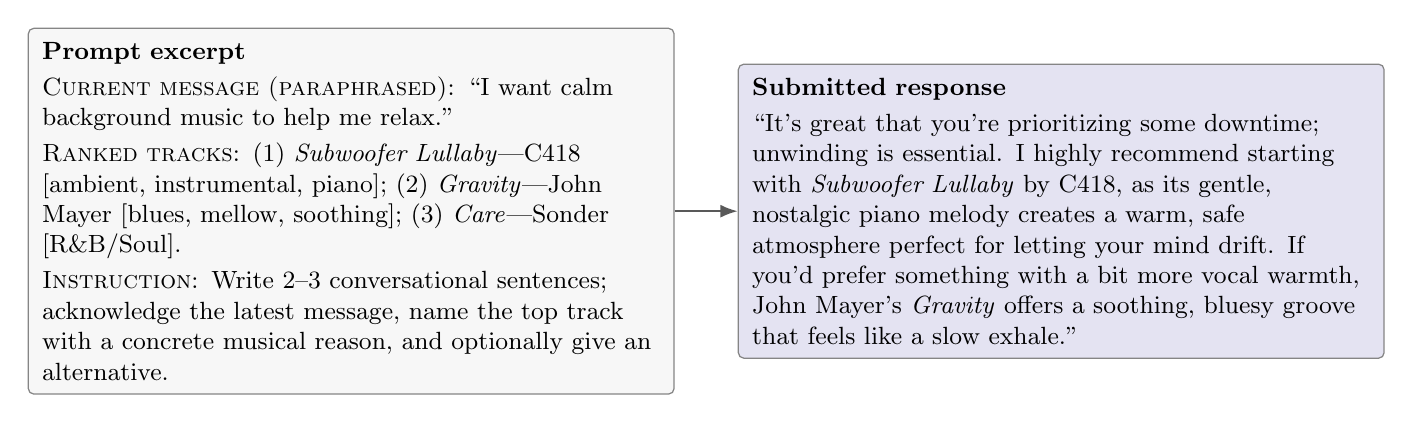
\begin{tikzpicture}[
  font=\small,
  example/.style={draw=black!48, line width=0.45pt, rounded corners=2pt,
    align=left, text width=78.5mm, inner sep=5pt,
    execute at begin node=\raggedright},
  exflow/.style={-{Latex[length=2.2mm]}, line width=0.7pt, draw=black!65},
]
  \node[example, fill=black!3] (prompt) {
    \textbf{Prompt excerpt}\\[2pt]
    \textsc{Current message (paraphrased)}: ``I want calm background music to
    help me relax.''\\[2pt]
    \textsc{Ranked tracks}: (1) \textit{Subwoofer Lullaby}---C418
    [ambient, instrumental, piano]; (2) \textit{Gravity}---John Mayer
    [blues, mellow, soothing]; (3) \textit{Care}---Sonder [R\&B/Soul].\\[2pt]
    \textsc{Instruction}: Write 2--3 conversational sentences; acknowledge
    the latest message, name the top track with a concrete musical reason,
    and optionally give an alternative.
  };
  \node[example, fill=respblue, right=8mm of prompt] (reply) {
    \textbf{Submitted response}\\[2pt]
    ``It's great that you're prioritizing some downtime; unwinding is
    essential. I highly recommend starting with \textit{Subwoofer Lullaby}
    by C418, as its gentle, nostalgic piano melody creates a warm, safe
    atmosphere perfect for letting your mind drift. If you'd prefer
    something with a bit more vocal warmth, John Mayer's \textit{Gravity}
    offers a soothing, bluesy groove that feels like a slow exhale.''
  };
  \draw[exflow] (prompt.east) -- (reply.west);
\end{tikzpicture}
\end{document}
